\section{Provas dos teoremas}
 
%%%%%%%%%%%%%%%%%%%%%%%%%%%%%%%%%%%%%%%%%%%%%%%%%%%%%%%%%%%%%%%%%%%%%%%%%%%%%%%%%%%%%%%
%%%%%%%%%%%%%%%%%%%%%%%%%%%%%%%%%%%%%%%%%%%%%%%%%%%%%%%%%%%%%%%%%%%%%%%%%%%%%%%%%%%%%%%
\begin{myproofT}[Prova do Teorema \ref{theo:minhxhx}]\label{proof:theo:minhxhx}
Dados,
um escalar $x \in \mathbb{R}$, 
um escalar $a \in \mathbb{R}$,  
uma função $h:\mathbb{R} \rightarrow \mathbb{R}$, e 
definida a Eq. (\ref{eq:proof:minhxhx0}),
\begin{equation}\label{eq:proof:minhxhx0}
e(x)=||h(x)-a||^2.
\end{equation}
Para achar o valor  $\hat{x}$ que gere o menor valor de $e(x)$, é aplicado
o critério que um ponto de inflexão $x^+$ (máximo, mínimo ou ponto de sela) de $e(x)$ 
pode ser achado quando 
$\left. \frac{\partial e(x)}{\partial x }\right|_{x=x^+} \equiv e'(x^+) =0$.
Assim, 
usando o Teorema \ref{theo:derfxbCfxb0} podemos 
rescrever esta igualdade como a Eq. (\ref{eq:proof:minhxhxe}),
\begin{equation}\label{eq:proof:minhxhxe}
2  h'(x) \left[h(x) -a\right] = e'(x)=0,
\end{equation}
Da Eq. (\ref{eq:proof:minhxhxe}), observamos 
que existem duas formas de achar um ponto de inflexão $x^+$,
\begin{itemize}
 \item a primeira forma a achamos se temos um valor $x^+$ tal que $h'(x^+)=0$, 
que representa um ponto de inflexão simultaneo em $e(x)$ e $h(x)$, e
 \item a segunda forma é achando um valor $x^+$ tal que $h(x^+)=a$;
que representa um ponto de inflexão de $e(x)$, mas não
necessariamente de $h(x)$; 
sendo este ponto $x^+=\hat{x}$ tambem um mínimo absoluto, pois provocam $e(\hat{x})=0$.
\end{itemize}




Por outro lado, podemos realizar uma aproximação linear de $h(x)$ em $e(x)$
ao redor do ponto $p$ usando a \hyperref[def:taylor]{\textbf{serie de Taylor}},
de modo que a Eq. (\ref{eq:proof:minhxhx0}) pode ficar expresada como
\begin{equation}\label{eq:proof:minhxhxe:approx0}
e(x) \approx  e_p(x) = ||h'(p)\{x-p\}-\{a-h(p)\}||^2.
\end{equation}
Assim, da Eq. (\ref{eq:proof:minhxhxe:approx0})
podemos concluir que um ponto $x^*$ que é 
um mínimo da aproximação linear $e_p(x)$ feita em $e(x)$ ao redor do ponto $\VECTOR{p}$,
pode ser achado como
\begin{equation}\label{eq:proof:minhxhx2}
 h'(p)\{x^*-p\} = \{a-h(p)\} \qquad \leftrightarrow \qquad x^* = p - \frac{h(p)-a}{ h'(p)}.
\end{equation} 

Desta equação podemos tirar a seguintes conclusões:
\begin{itemize}

\item Observamos que a posição $p$ é corregida para ficar próximo à posição $x^*$, 
que é um mínimo absoluto de $e_p(x)$ na direção de um mínimo (qualquer) de $e(x)$;
pelo que se deduz que a Eq. (\ref{eq:proof:minhxhx2})
pode ser usada para procurar aproximações $x^*$ de pontos mínimos $\hat{x}$ em $e(x)$ desde a posição $p$;
ou pelo menos aproximações de novas posições em caminhos numa direção descendente de $e(x)$.

\item A Eq. (\ref{eq:proof:minhxhx2}) é satisfeita 
com $x^* \approx p$ se acharmos um  
ponto $p$ onde  $a \approx h(p)$; 
é dizer um mínimo global de $e(x)$ em $p$.%, como pode ser visto na Figura \ref{fig:ex0a}. 

\item Dado que a Eq. (\ref{eq:proof:minhxhx2}) avança desde $p$ na direção de um mínimo $x^*$, 
mesmo que nos pontos de inflexão $x^+$ correspondentes a máximos ou pontos de sela,
encontremos valores de $p$ próximos a $x^*$,
 estes casos serão pouco estáveis pois
a correção da posição $p$ será na direção de um mínimo e não do máximo.

\item Se modificamos a Eq. (\ref{eq:proof:minhxhx2}), e escolhemos um ponto  
$p_0$ que consideremos próximo ao ponto $\hat{x}$ que minimiza $e(\hat{x})$,
podemos achar iterativamente aproximações lineares $x^*$ cada vez mais próximos a  $\hat{x}$,
se usamos a seguinte equação iterativa,
\begin{equation}\label{eq:proof:minhxhx3}
p_{k} \leftarrow p_{k-1} - \frac{ h(p_{k-1})-a}{h'(p_{k-1})},
\end{equation}
iniciando desde um $p_{0}$ 
ate que exista uma tendencia prolongada onde se observe que $p_{k}$ é muito próximo a $p_{k-1}$,
momento no qual declaramos que $\hat{x} \approx p_{k}$.
\item Pode existir um mínimo global $\hat{x}$ de $e(\hat{x})>0$.
Isto nos restringe a que no uso da Eq. (\ref{eq:proof:minhxhx3}),
nosso critério principal para estabelecer o final do cáculo iterativo,
deve ser a tendencia na  proximidade entre $p_{k}$ e $p_{k-1}$ 
e não o valor de $e(x_k)$.
\end{itemize}

Um diagrama completo resumindo todas estas conclusões pode ser visto na Figura \ref{fig:fluxohx1}.
\end{myproofT}



\begin{figure}[!h]
     \centering
         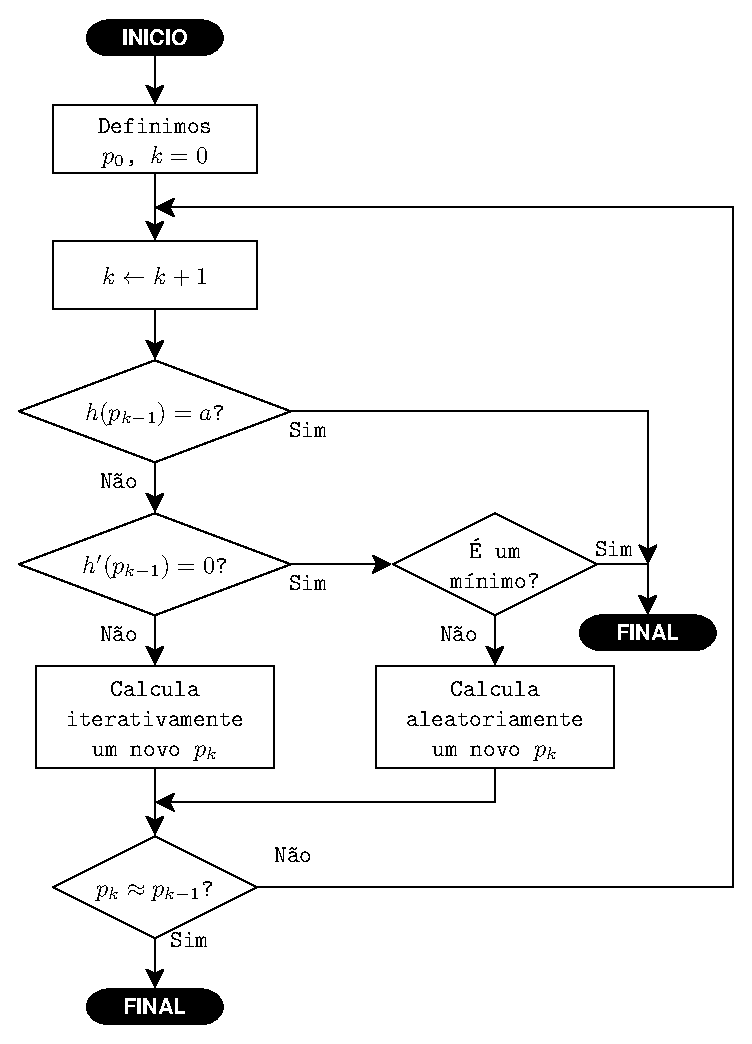
\includegraphics[width=0.75\textwidth]{chapters/minimization-hx/fluxo1.eps}
        \caption{Diagrama de fluxo da solução iterativa para achar um mínimo, seguindo a Prova \ref{proof:theo:minhxhx}.}
        \label{fig:fluxohx1}
\end{figure}


%%%%%%%%%%%%%%%%%%%%%%%%%%%%%%%%%%%%%%%%%%%%%%%%%%%%%%%%%%%%%%%%%%%%%%%%%%%%%%%%%%%%%%%
%%%%%%%%%%%%%%%%%%%%%%%%%%%%%%%%%%%%%%%%%%%%%%%%%%%%%%%%%%%%%%%%%%%%%%%%%%%%%%%%%%%%%%%
\begin{myproofT}[Prova do Teorema \ref{theo:minhxhxxbxb}]\label{proof:theo:minhxhxxbxb}
Dados,
um escalar $x \in \mathbb{R}$, 
um escalar $a \in \mathbb{R}$,
um escalar $\alpha \in \mathbb{R}^{+}$,
um escalar $b \in \mathbb{R}$,
uma função $h:\mathbb{R} \rightarrow \mathbb{R}$, e 
definida a Eq. (\ref{eq:proof:minhxhxxbxb0}),
\begin{equation}\label{eq:proof:minhxhxxbxb0}
e(x)=||h(x)-a||^2+\alpha ||x-b||^2.
\end{equation}
Para achar o valor  $\hat{x}$ que gere o menor valor de $e(x)$, é aplicado
o critério que um ponto de inflexão (máximo, mínimo ou ponto de inflexão) de $e(x)$ pode ser achado quando 
$\left. \frac{\partial e(x)}{\partial x }\right|_{x=\hat{x}} \equiv e'(\hat{x}) =0$.
Assim, 
usando o Teorema \ref{theo:derfxbCfxb0} e \ref{theo:derAxbAxb} podemos 
rescrever esta igualdade como a Eq. (\ref{eq:proof:minhxhxxbxbe}),
\begin{equation}\label{eq:proof:minhxhxxbxbe}
2  h'(x) \left[h(x) -a\right]+2\alpha (x-b)= e'(x)=0,
\end{equation}
Da Eq. (\ref{eq:proof:minhxhxxbxbe}), observamos 
que existem duas formas de achar um ponto de inflexão em $e(x)$,
\begin{itemize}
 \item a primeira é sim $h'(x)$ tem um fator $(x-b)$ tal que $h'(b)=0$, e
 \item a segunda forma é achando um valor $\hat{x}$ tal que $e'(\hat{x})=0$;
\end{itemize}
de isto se deduz que se $h'(x)$ tem um fator $(x-b)$ então, $x=b$ representa um ponto de inflexão de $e(x)$ e $h(x)$;
porem, existe um ponto $\hat{x}$ que provoca $e'(\hat{x})=0$, representa um ponto de inflexão de $e(x)$, exclusivamente. 
Assim, dada a natureza positiva de $e(x)$,este é obrigatoriamente um mínimo global de $e(x)$.

Por outro lado, usando o Teorema \ref{theo:derfxbCfxbxqDxq} podemos 
rescrever a Eq. (\ref{eq:proof:minhxhxxbxbe}) de forma aproximada como a Eq. (\ref{eq:proof:minhxhxxbxb1}),
\begin{equation}\label{eq:proof:minhxhxxbxb1}
2  h'(p) \left[\left(h(p)-a\right) + h'(p) \left(\hat{x} - p\right)\right] \approx
e'(\hat{x})=0.
\end{equation}
de modo que, se consideramos $h'(p)\neq 0$, a equação pode ser rescrita como:
%um ponto de inflexão $\hat{x}$ de $e(x)$ pode ser achado aproximadamente quando:
\begin{equation}\label{eq:proof:minhxhxxbxb2}
\hat{x} \approx p - \frac{\left(h(p)-a\right)}{h'(p)}.
\end{equation}
Isto quer dizer que a Eq. \ref{eq:proof:minhxhxxbxb2}, \textbf{serve só para
achar pontos de inflexão de} $e(x)$ \textbf{que não pertençam a} $h(x)$.
Sendo este obrigatoriamente um ponto onde $h(\hat{x})-a\approx 0$, 
equivalente a um mínimo global.

Assim, quanto mais próximo a $\hat{x}$ seja  o valor $p$, 
a Eq. (\ref{eq:proof:minhxhxxbxb2}) fica mais próximo a uma igualdade. Por outro lado,
a equação nos indica que dado um ponto  $p$ qualquer,
$p - \left[ h'(p) \right]^{-1}\left(h(p)-a\right)$
é um ponto próximo de $p$  na direção de um mínimo de $e(x)$.
De modo que, um bom critério para procurar um mínimo é seguir a seguinte 
equação iterativa,
\begin{equation}\label{eq:proof:minhxhxxbxb3}
p_{k} \leftarrow p_{k-1} - \frac{ \left(h(p_{k-1})-a\right)}{h'(p_{k-1})},
\end{equation}
iniciando desde um $p_{0}$ qualquer, ate que $p_{k}$ seja muito próximo a $p_{k-1}$,
onde se declara que $\hat{x} \approx p_{k}$. 


porem deve-se ter cuidado com valores de $p_{k}$ que provoquem 
$0<|h'(p_{k})|<\lim\limits_{\varepsilon \rightarrow +0}\varepsilon$,
pois estes valores tendem a divergir. Por outro lado sim se acha um valor 
de $p_{k}$ com $h'(p_{k})= 0$, deve ser
corroborado se este ponto tratasse de um máximo ou mínimo, local ou global, ou ponto de inflexão;
usando algum método, por exemplo estudando o comportamento 
de $e(x)$ ou analisando a matriz hessiana de $e(x)$ avaliada em $p_{k}$.

\end{myproofT}
